% Chapter 3

\chapter{Design} % Main chapter title

\label{Chapter3} % For referencing the chapter elsewhere, use \ref{Chapter1} 

\lhead{Chapter 3. \emph{Design}} % This is for the header on each page - perhaps a shortened title

%----------------------------------------------------------------------------------------

% \emph{How the product was designed, with discussion of design alternatives (referring to Appendix B for details).}
% 
% \emph{Diskuter de viktigste funksjonene i ditt design og hvordan det har utviklet seg, fremhev noen nye/originale funksjoner.}
% 
% \emph{Ikke ha med design dokumentasjon her!}

The basic architecture is outlined in figure~\ref{fig:1_basic_architecture}. Our work will be aimed at the component labelled \emph{A}.

\begin{figure}[h]
  \centering
    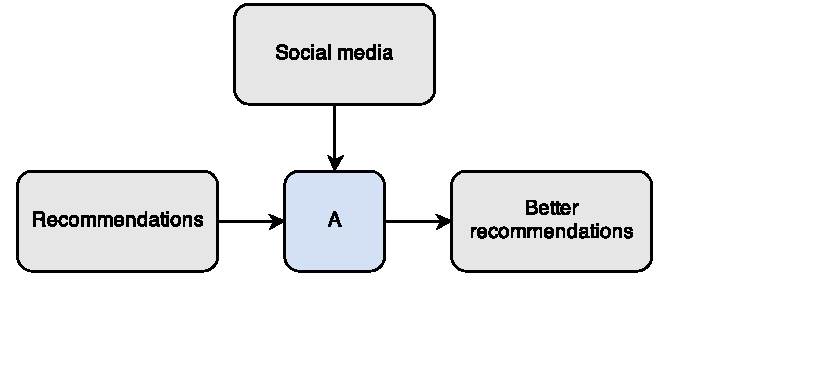
\includegraphics{Figures/01-high-level-architecture}
  \caption{The basic architecture of a system described in this thesis. We mainly describe the component labelled \emph{A}.}
  \label{fig:1_basic_architecture}
\end{figure}

The \emph{A} component is structured as illustrated in figure~\ref{fig:2_component_architecture}.

\begin{figure}[h]
  \centering
    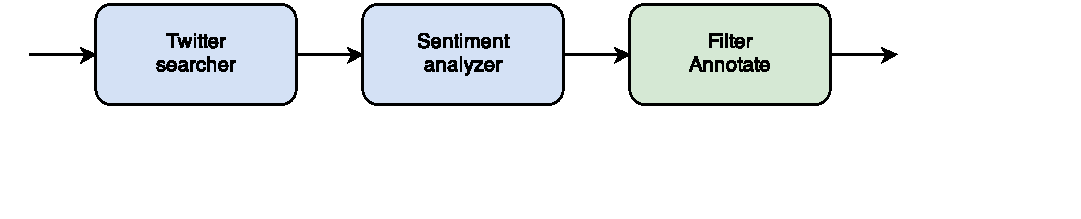
\includegraphics{Figures/02-component-layout}
  \caption{The layout of the system within component A.}
  \label{fig:2_component_architecture}
\end{figure}

